\chapter{Implementation}

This chapter covers in detail the implementation of the features covered within the design chapter and will list in detail the general implementation of a feature including their issues. It will also detail the environments and tools used to create the application and the supporting services behind the application.

\section{Tools used}

In this section the tools used for building the application and backend services will be detailed and their role within the development of the project as a whole.

\subsection*{Sublime Text}

Sublime Text is one of the main tools that was used throughout the development of the project. It is highly regarded as one of the best text editors in the public space due to its flexibility and community support to help it fit the user's needs.\\
\\
It has been a crucial tool for developing the middle tier application as all of the code was written in sublime text. This very report was exclusively written in Sublime Text and the vast majority of the SQL was also written within the Sublime Text editor. An image of the text editor can be found in figure \ref{fig:sublime_text_image}.

\begin{figure}[H]
    \centering
    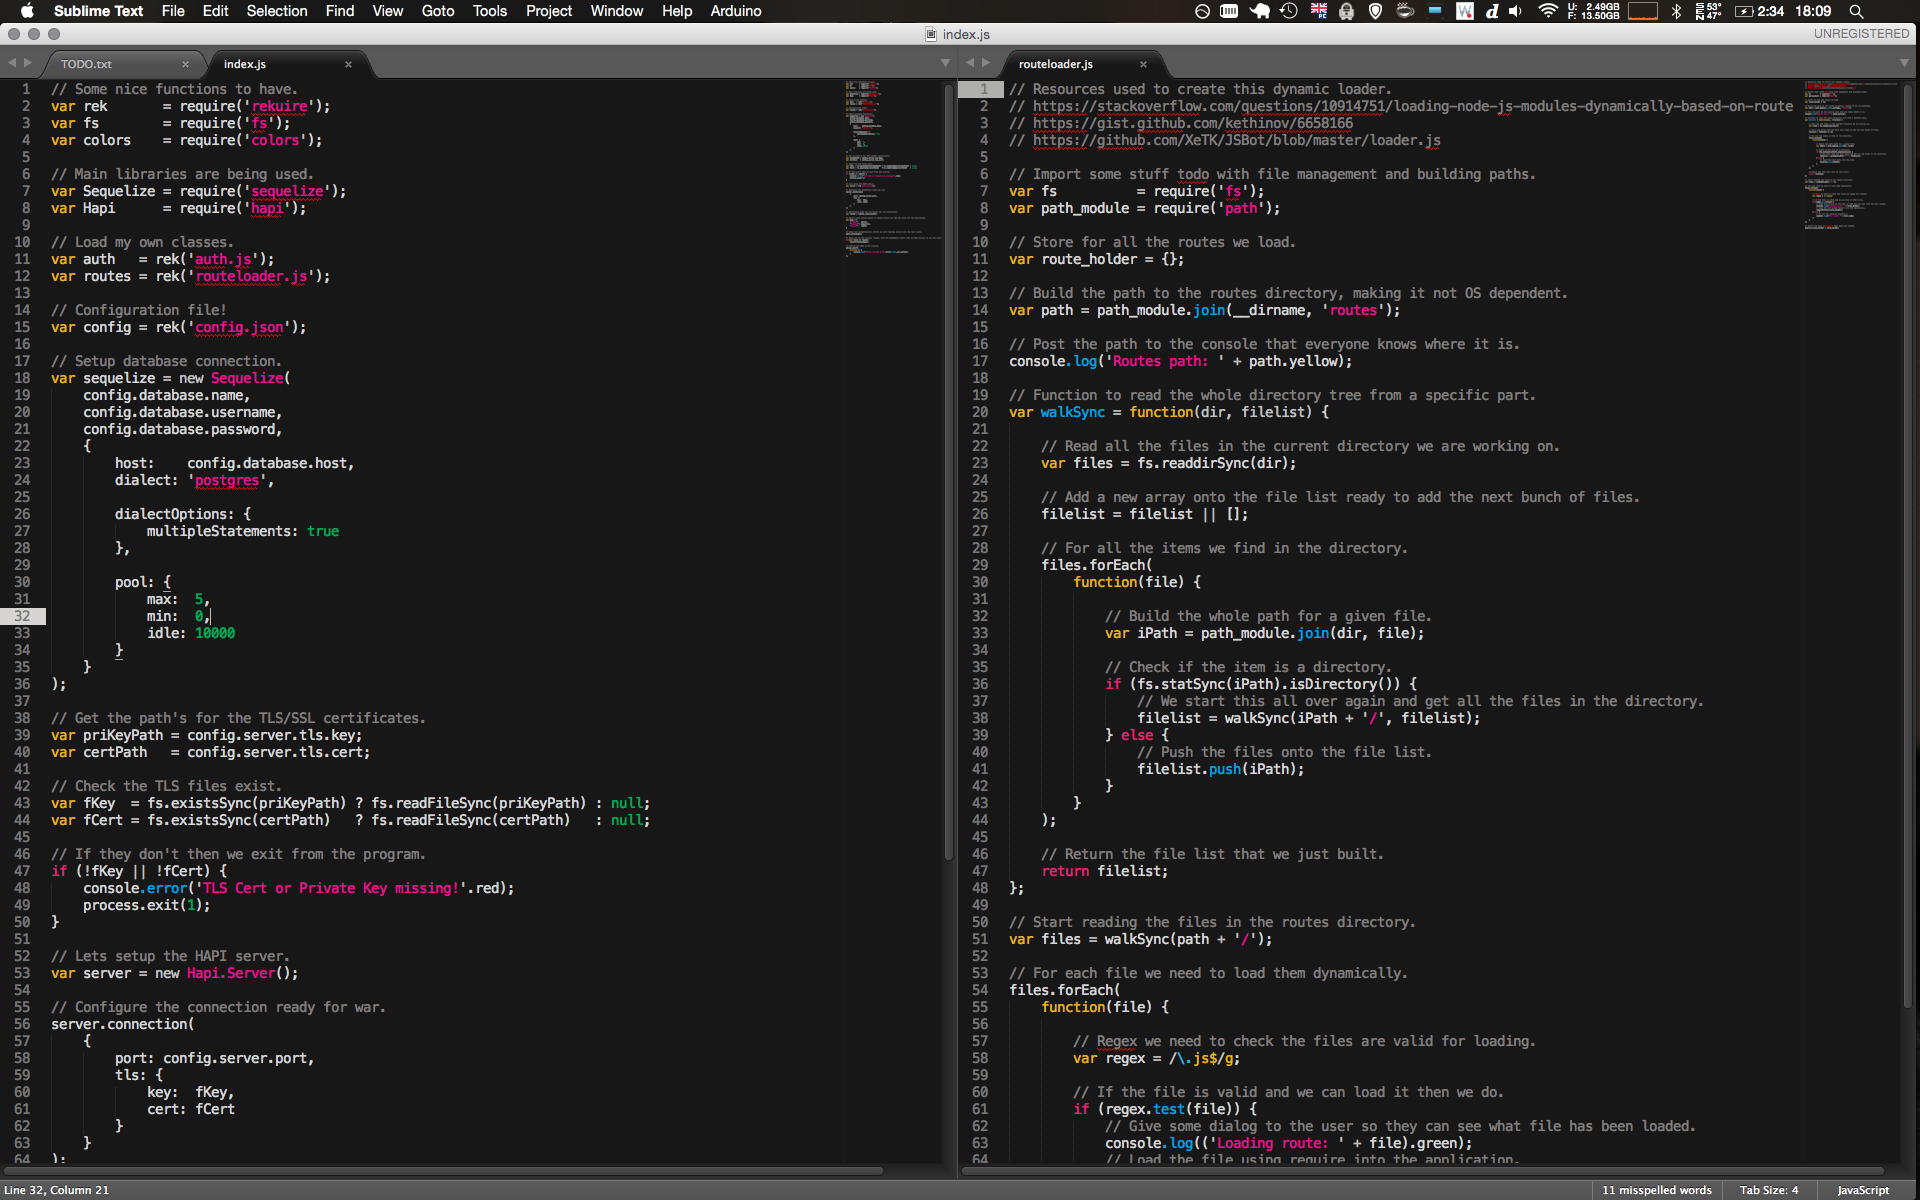
\includegraphics[width=\textwidth]{tools/sublime}
    \caption{Sublime Text 3.0}
    \label{fig:sublime_text_image}
\end{figure} 

\subsection*{Android Studio}

Android Studio has played the most crucial role within the development of the project. It has been the integrated development environment of choice for Android development, giving all the required features and tools needed to create a fully fledged Android application with the potential of being released into a production environment. It contains all of the testing tools required to do good Android development with a unit testing suite and various UI testing suites.\\
\\
It has close links to the Android SDK so it enables users to use the various Android SDK tools within the Android Studio GUI. Some of the advanced tools within the Android SDK are covered later in this section. Android Studio offers powerful code completion tools and refactoring tools to speed up the development of the application. It also has the ability to error check the code and provide solutions through the development of the project, with powerful auto complete tools to build up the stub functions to complete the implementation of imported libraries. An example of the layout and design of Android studio can be found in figure \ref{fig:android_studio_image}.

\begin{figure}[H]
    \centering
    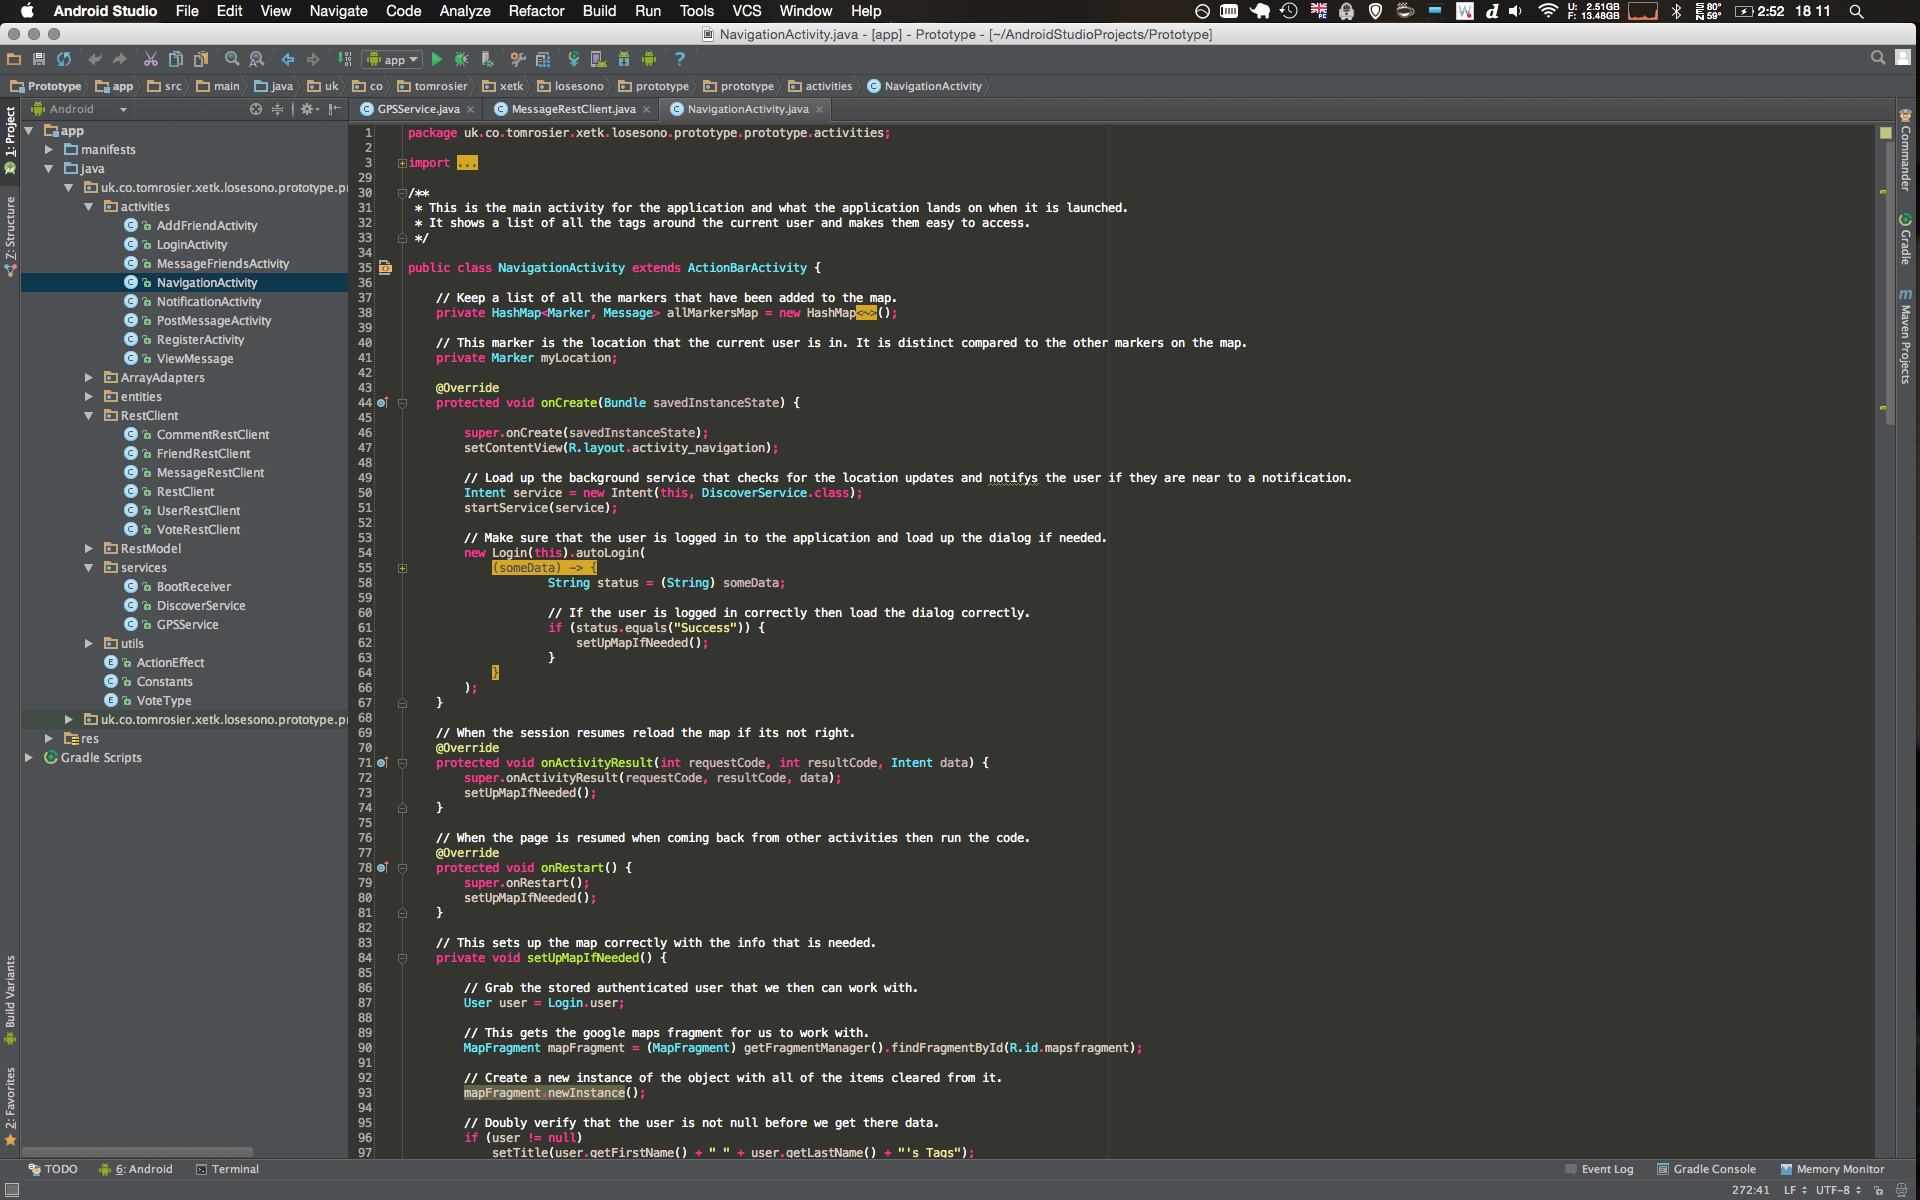
\includegraphics[width=\textwidth]{tools/androidstudio}
    \caption{Android Studio 1.1.0}
    \label{fig:android_studio_image}
\end{figure} 

\subsection*{PGAdmin3}

PGAdmin3 is a tool for remotely accessing Postgres database and allowing management through a GUI based interface. It allows easy access to viewing data held within the database, along with the ability to execute SQL commands directly on the database. The tool was mostly used as a verifier to check that SQL executed within the terminal had run correctly and had created the tables and constraints that were needed for the application to work correctly. Small note; this crashes a lot on a Apple Mac. An example of the execution of PGAdmin3 can be found in figure \ref{fig:pg_admin_image}.

\begin{figure}[H]
    \centering
    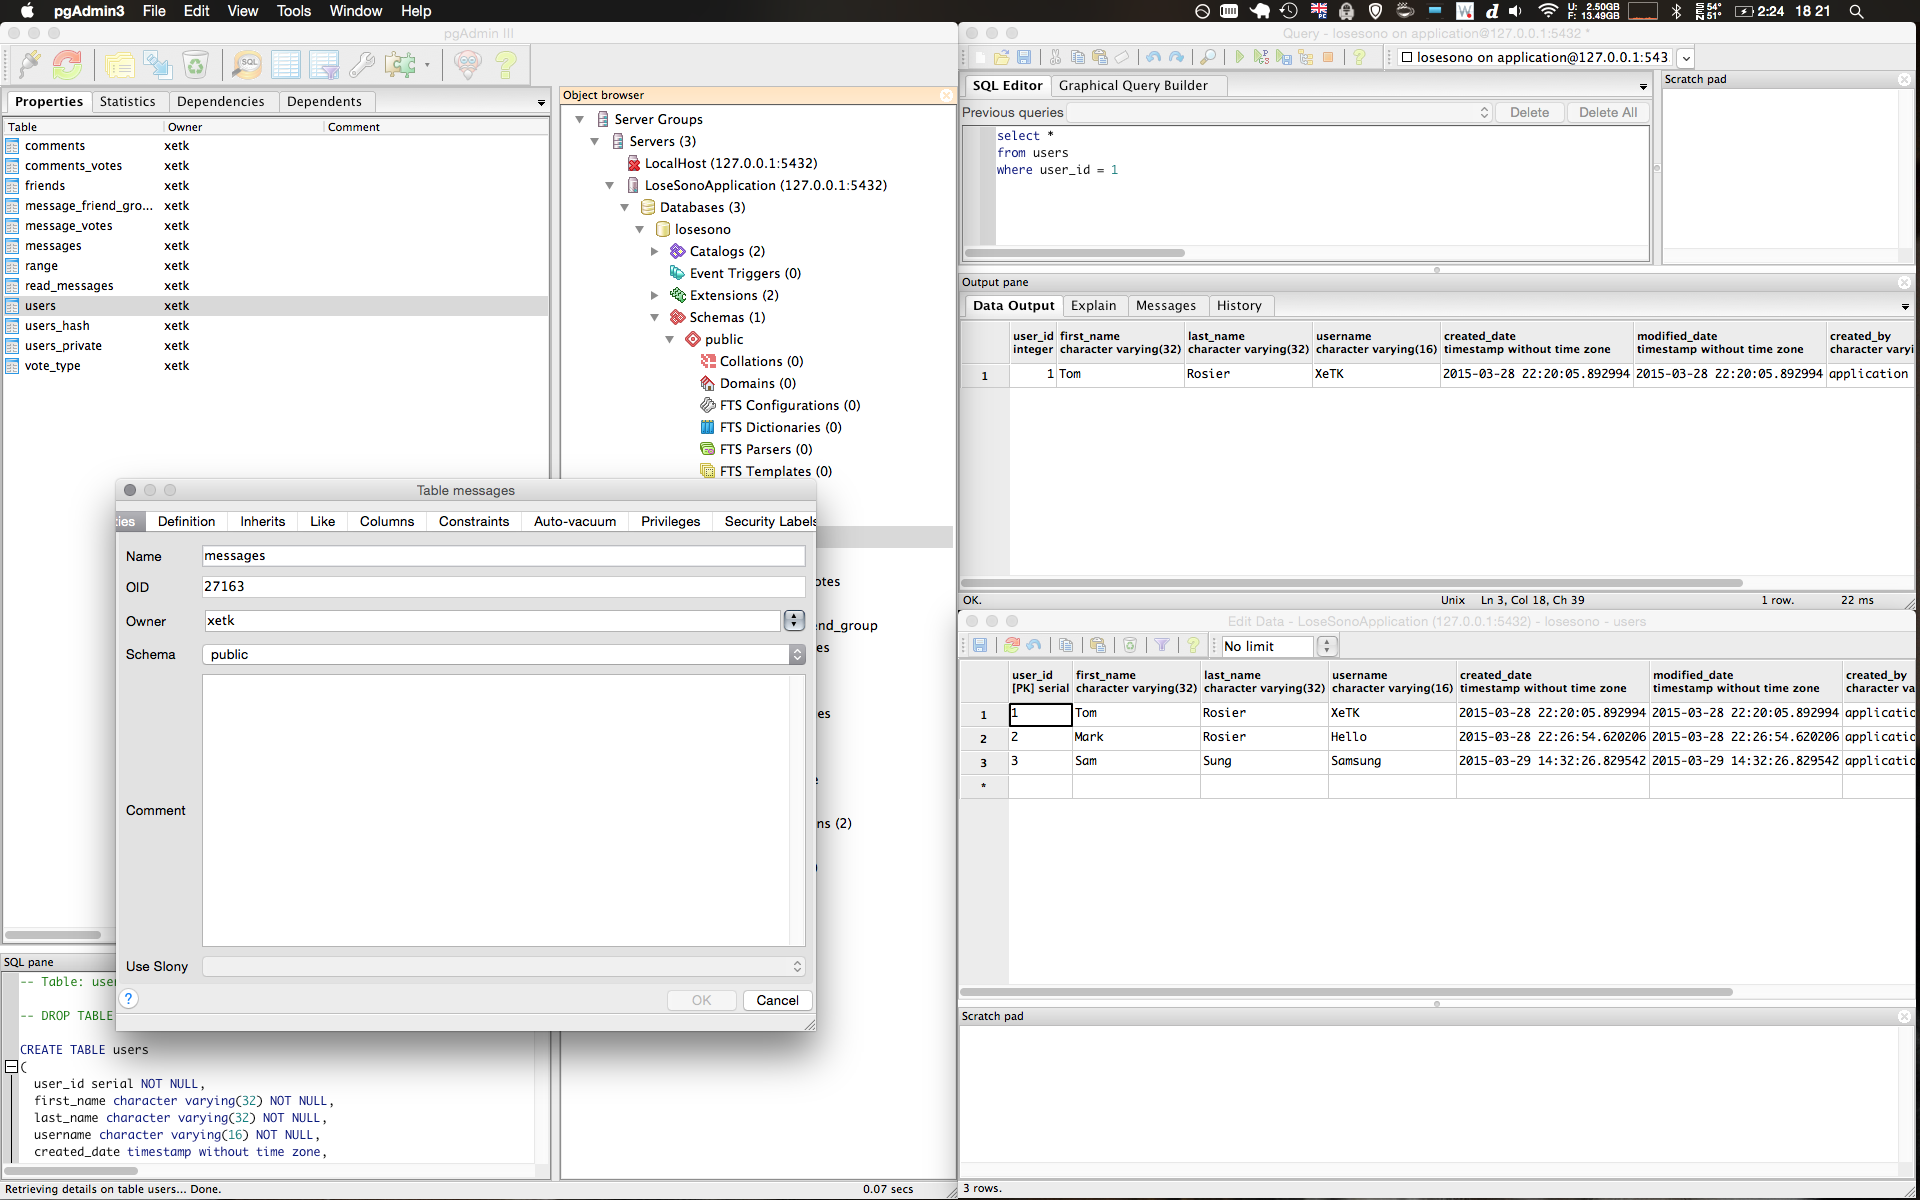
\includegraphics[width=\textwidth]{tools/pgadmin}
    \caption{PGAdmin3 1.20.0}
    \label{fig:pg_admin_image}
\end{figure} 

\subsection*{PGSQL command line}

The PostgreSQL command line tool was used in conjunction with PGAdmin3 to do all the SQL related work needed for the project. The PostgreSQL command line allows direct command execution within the SQL engine, so is perfect for debugging issues within the database, along with creating the SQL statements to extract the data needed to get the functional requirements of the application working correctly.\\
\\
PostgreSQL itself is fairly difficult to install correctly and there were many issues with getting it to install and work as intended. The command line package manager for Apple Mac; Homebrew PostgreSQL's package, is completely broken and caused massive headaches at the start of the project. These issues were resolved by installing the official DMG package provided by Postgres.app \cite{jemt:postgresapp:2015:online}.

\begin{figure}[H]
    \centering
    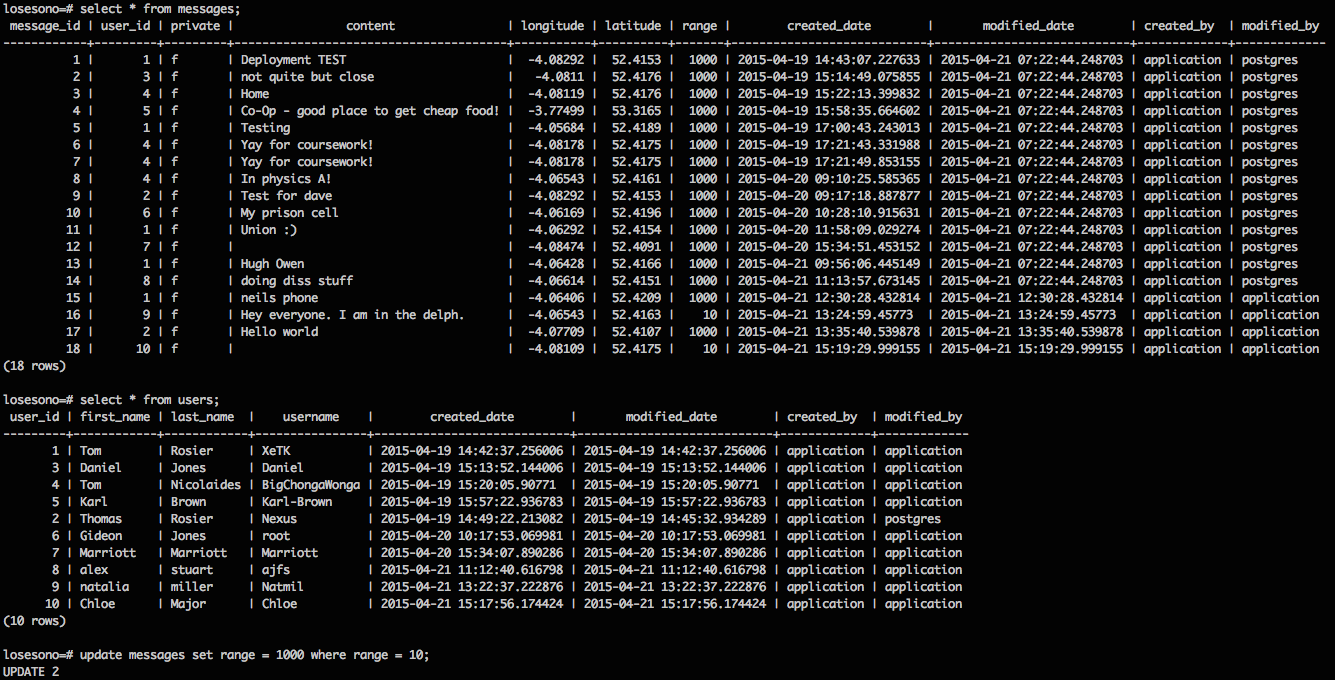
\includegraphics[width=\textwidth]{tools/pgsqlcommandline}
    \caption{PG SQL Command line 9.3.6}
    \label{fig:pg_sql_image}
\end{figure} 

\subsection*{Postman}

Postman was an essential tool for debugging the RESTful interfaces provided by the applications. It enables the emulation of HTTP POST and GET requests enabling the ability to attach the parameters needed when completing a POST request and making sure the interface is working correctly without the need to implement it fully into the application. It was often used to check if the RESTful interface was working correctly before implementing the corresponding code within the Android side of the application. Postman itself has a few issues. If a request would fail,for whatever reason, the application would get stuck in the sending request stage and would require closing the tab and re-opening. An image of Postman at work can be found in figure \ref{fig:postman_image}.

\begin{figure}[H]
    \centering
    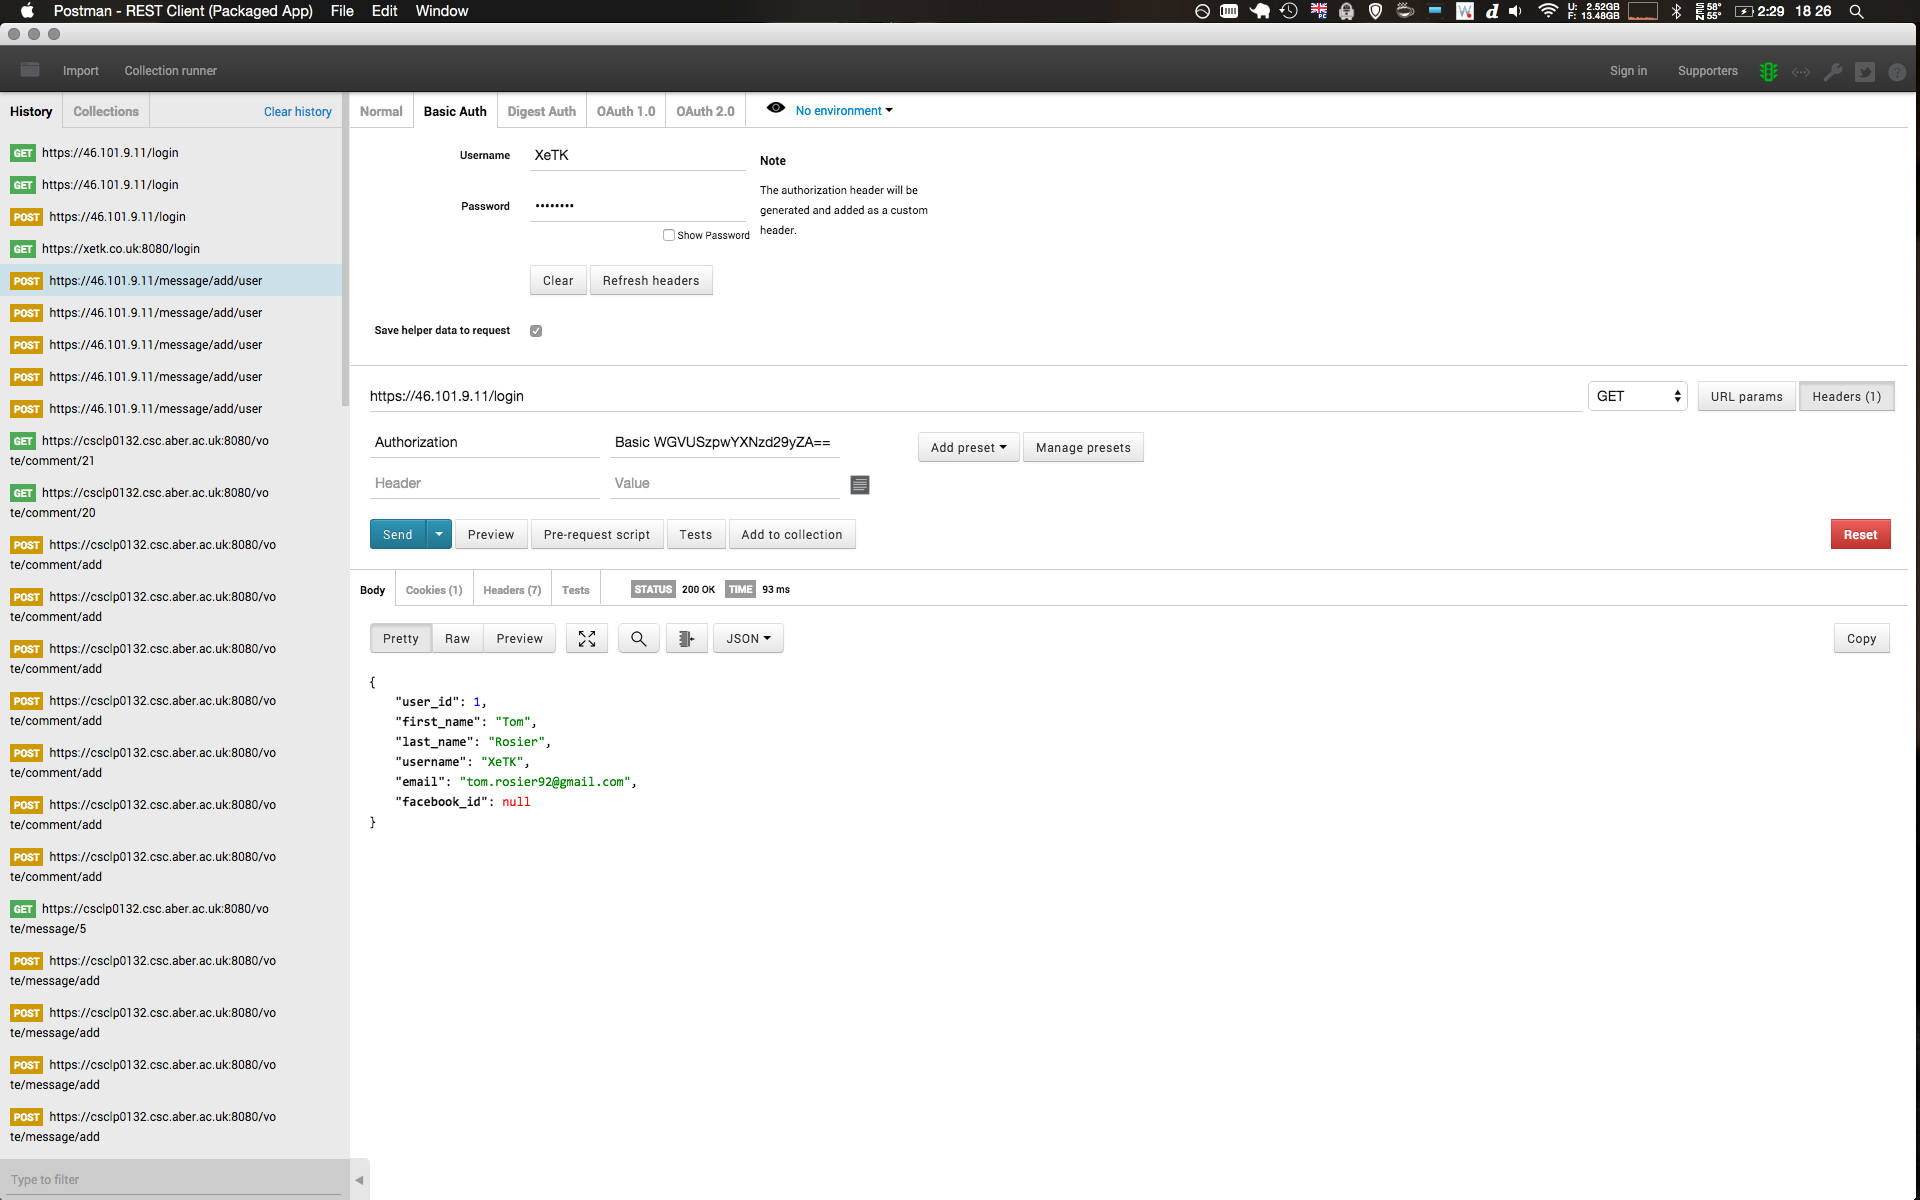
\includegraphics[width=\textwidth]{tools/postman}
    \caption{Postman 2.0.19}
    \label{fig:postman_image}
\end{figure} 

\subsection*{Web browsers}

A web browser is an essential tool in any software related tool in the modern world. It was primarily used for researching the project as a whole but it was also used for debugging the backend API as it can carry out HTTP requests, accept cookies and deal with HTTP authentication. They were often used to complement Postman when it could not quite carry out the required action that was needed.\\
\\
The two main browsers used to test the application were Opera And Google Chrome, Opera being my main browser, so Chrome was used as a backup when needed. Images of the two main browsers that were used can be found in figures \ref{fig:opera_image} and \ref{fig:chrome_image}.

\begin{figure}[H]
    \centering
    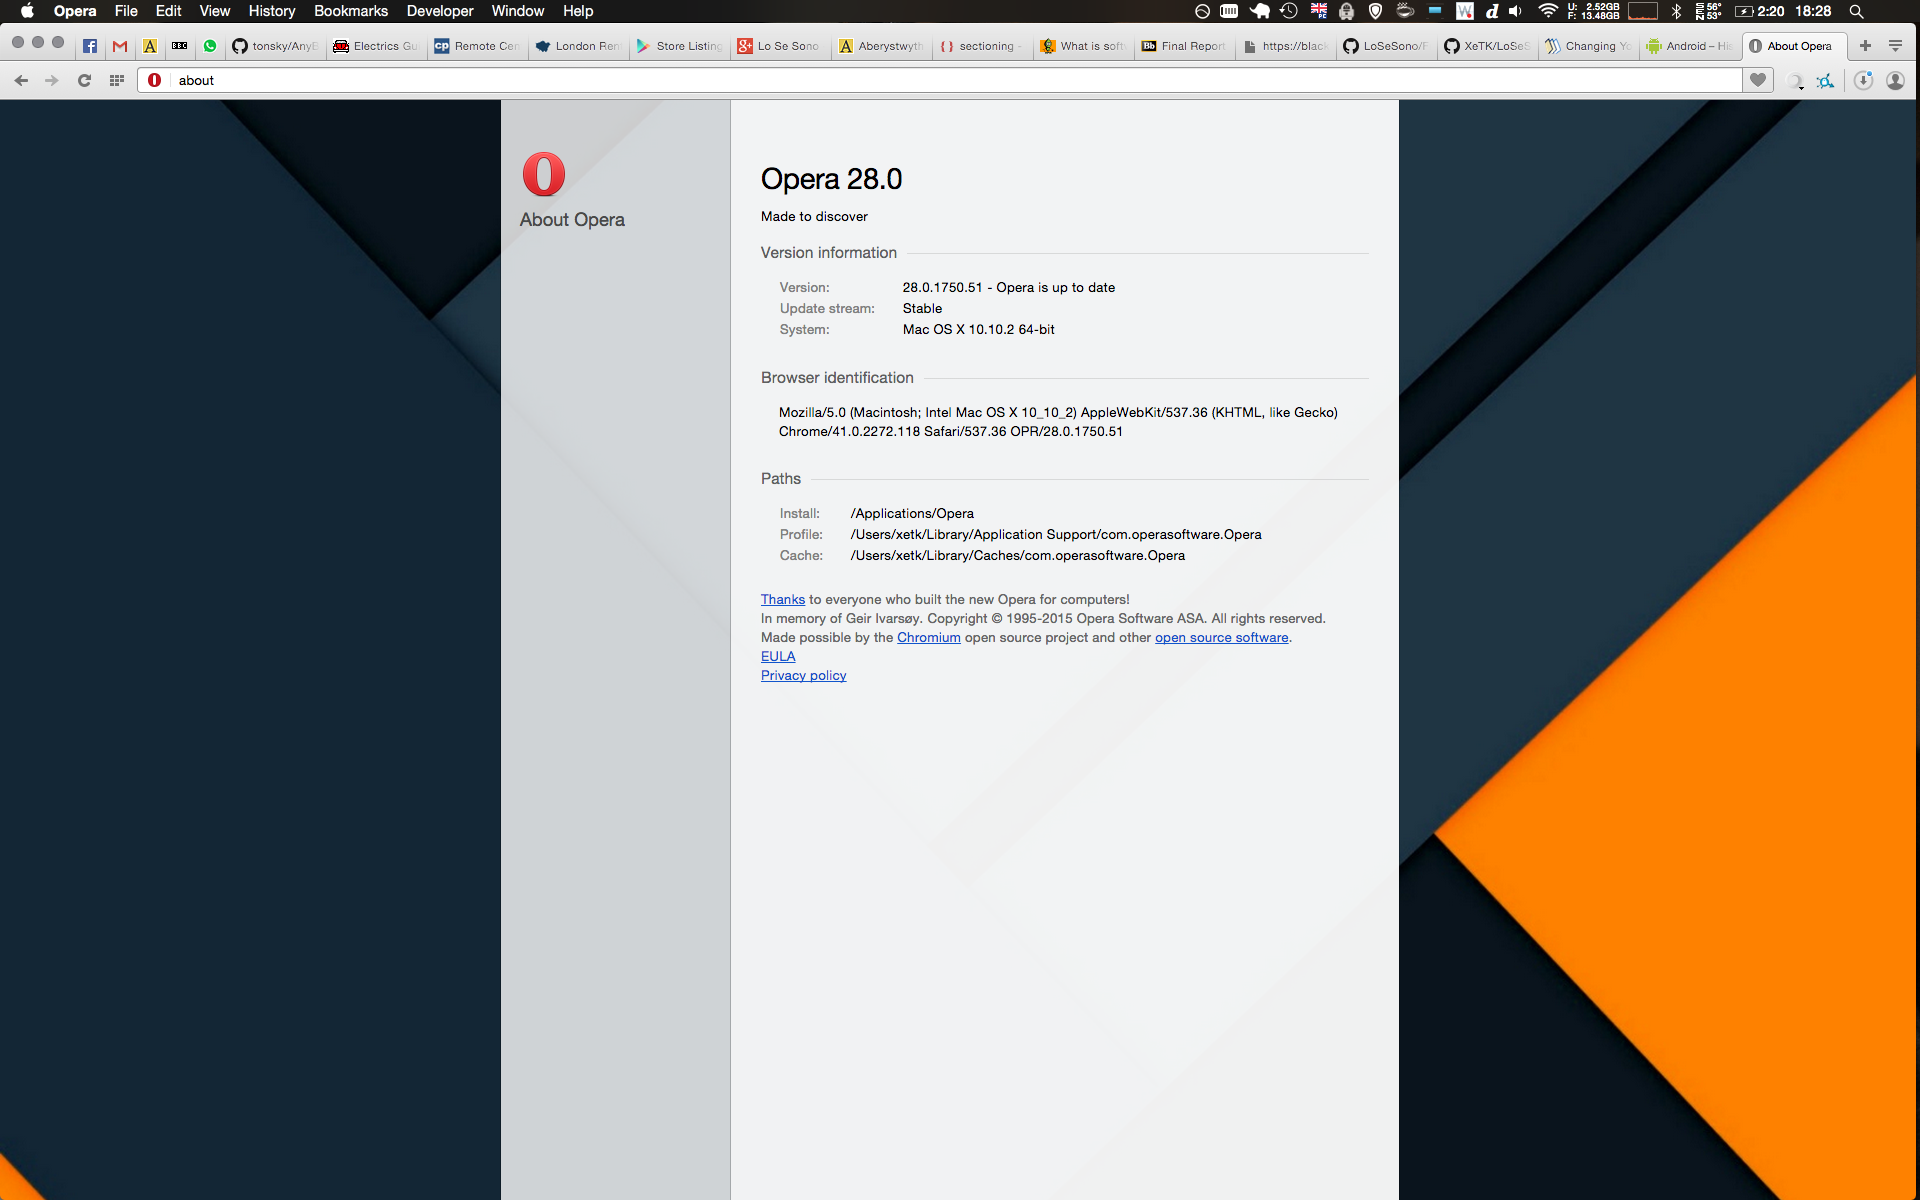
\includegraphics[width=\textwidth]{tools/opera}
    \caption{Opera 28.0}
    \label{fig:opera_image}
\end{figure} 

\begin{figure}[H]
    \centering
    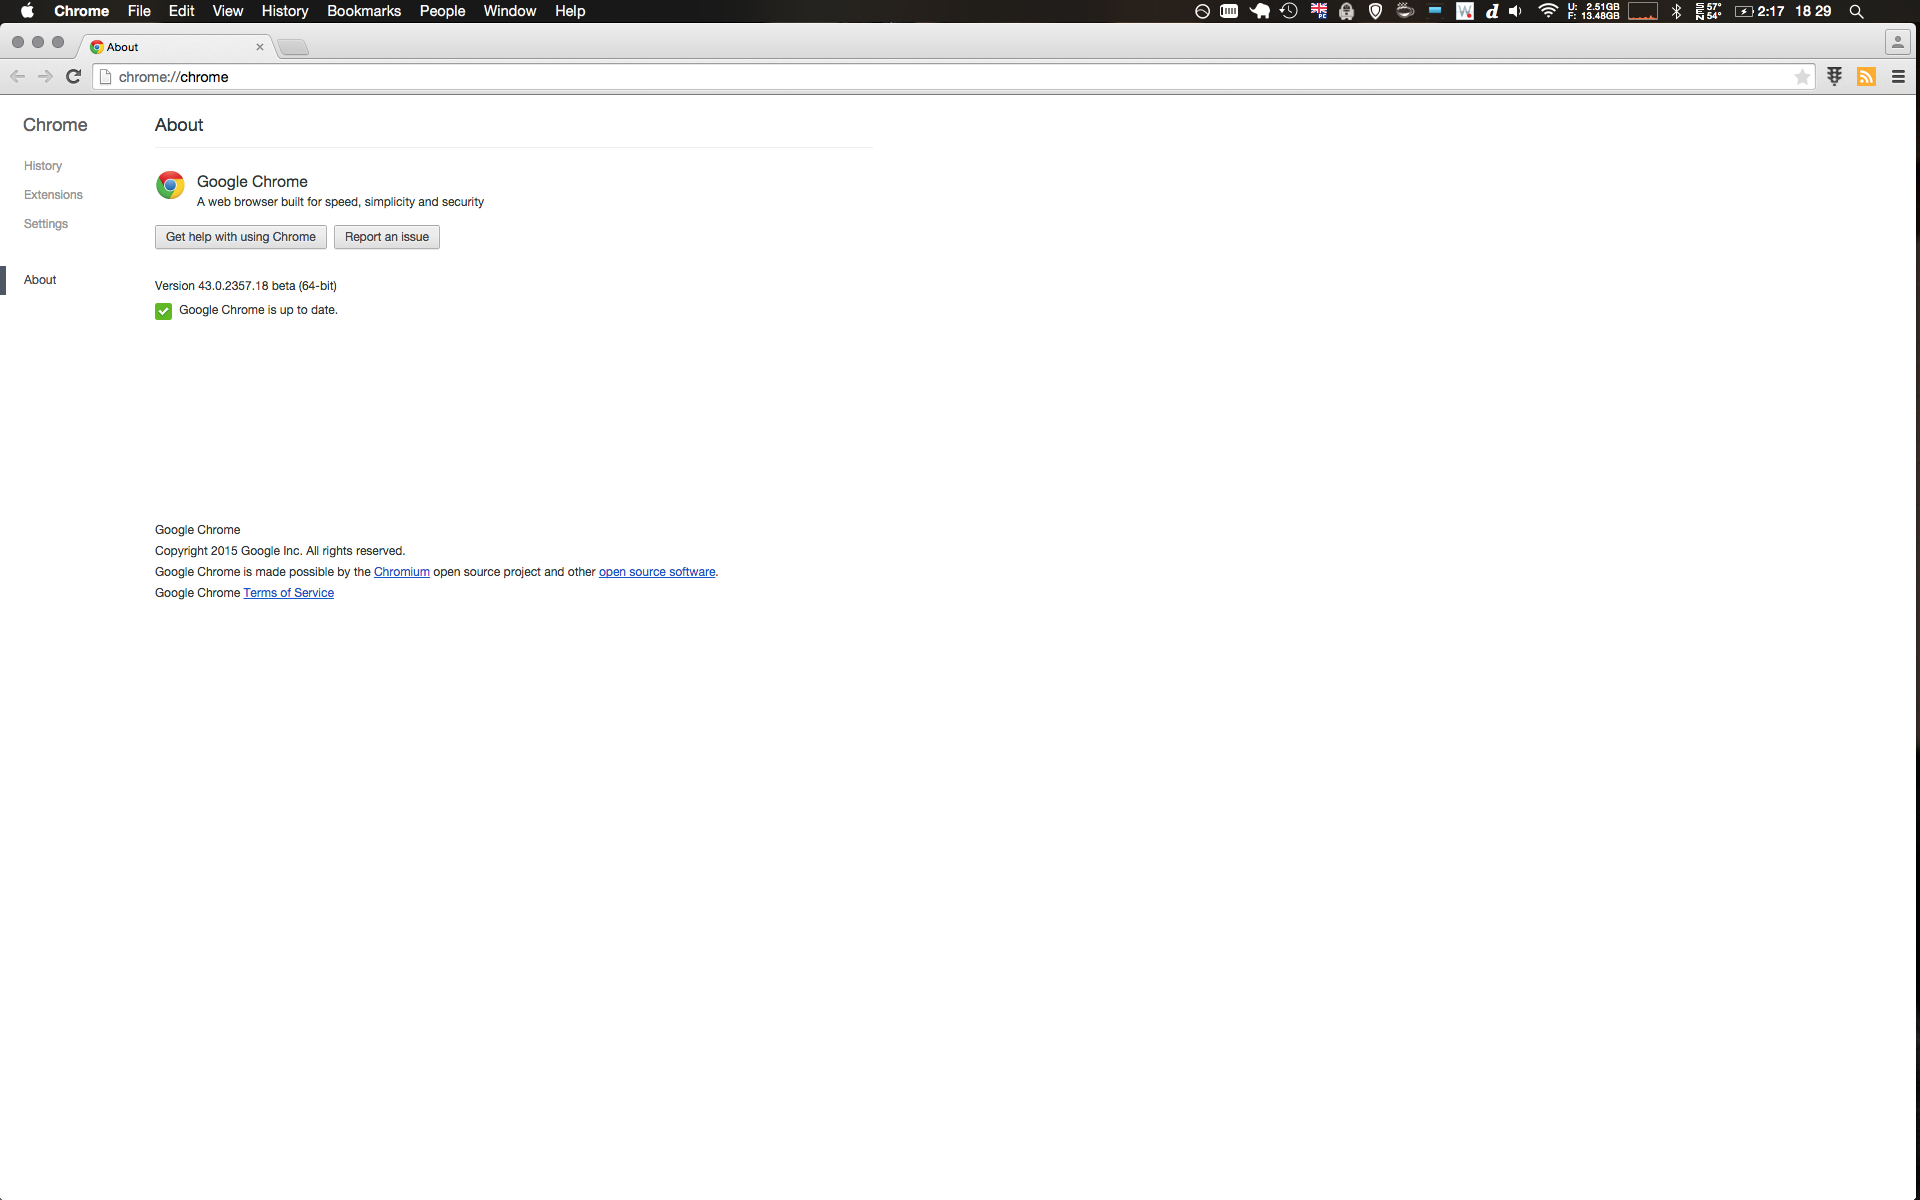
\includegraphics[width=\textwidth]{tools/chrome}
    \caption{Chrome 43.0}
    \label{fig:chrome_image}
\end{figure} 

\subsection*{Android SDK Tools}

Throughout the development of the project there was a need to use the full Android Software Development Kit for testing and debugging the application in the given environment in which it would run. The SDK provides all of the build tools needed to create and compile the packages needed to install the application on the device, along with submitting it to the Google Play Store.\\
\\
The first and possibly most used tool throughout the development of the application is the Android Emulator. This tool emulates the Android platform on the development machine to provide an environment to test code without the need of a physical device. This can be useful when the developer only has a limited selection of devices to test the application on, as the emulator gives the ability to scale to different screen sizes and resolutions to help with debugging on different devices. In figure \ref{fig:android_emulator} shows the emulator at work running the application in a test mode.

\begin{figure}[H]
    \centering
    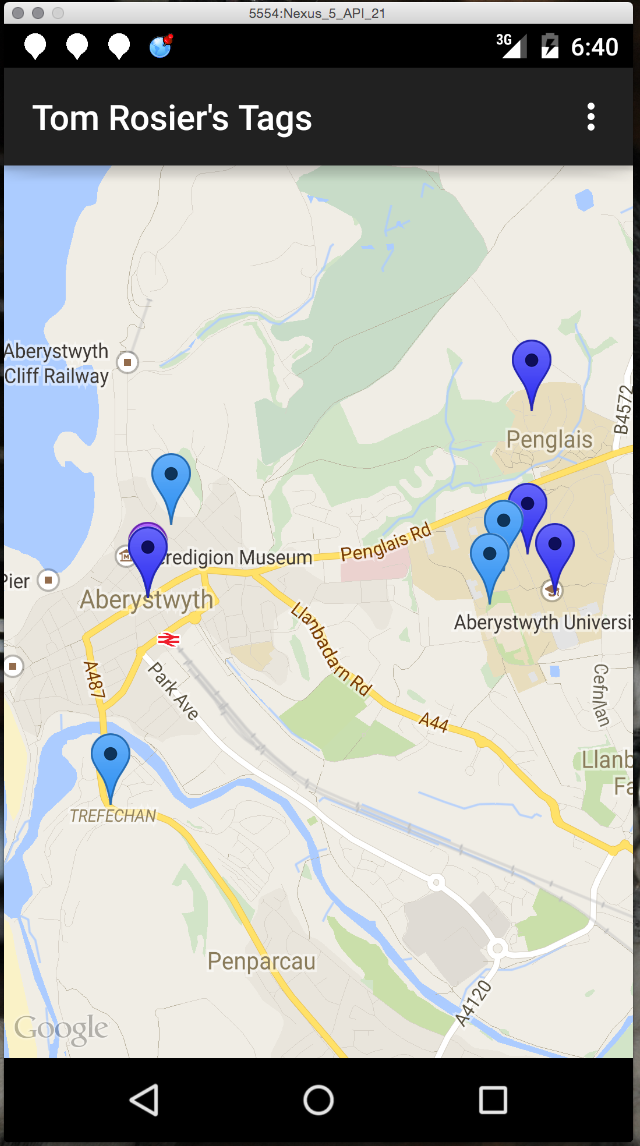
\includegraphics[width=0.5\textwidth]{tools/androidemulator}
    \caption{Android Emulator SDK 22}
    \label{fig:android_emulator}
\end{figure} 

\label{sec:adb}
\noindent
Another equally important tool that was used extensively during the development of the project was the command line application Android Development Bridge (ADB). ADB is used to interface with Android based devices and provides many features that allow interfacing and connecting to the device. It is crucial for debugging applications along with working with the Operating System directly. It has been extensively used throughout this project to repair damaged and broken phones to bring them back to a state where they can be used to help with development.

\begin{figure}[H]
    \centering
    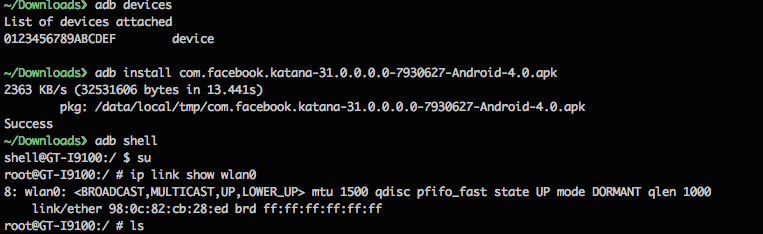
\includegraphics[width=0.75\textwidth]{tools/adb}
    \caption{Android Development Bridge}
    \label{fig:adb_image}
\end{figure} 

\noindent
The SDK updater played a very minor role in the project, but it allows an easy and quick way to update the SDK and build tools within the Android development suite to the latest versions to enable development for newer devices as they come to market.

\begin{figure}[H]
    \centering
    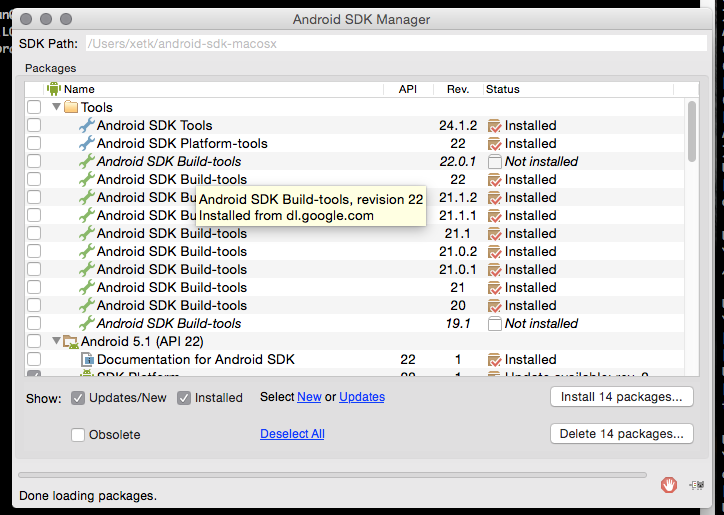
\includegraphics[width=0.75\textwidth]{tools/sdkupdator}
    \caption{Android SDK Updater}
    \label{fig:sdk_updator}
\end{figure} 

\subsection*{Git Hub}

Throughout the project the version control system GIT has been used to ensure that the source code for the project has been reliably backed up and provides the ability to check in versions of the code to return to a prior point if needed.\\
\\
The use of the service GitHub as an on-line repository allows the code to be kept easily accessible and backed up throughout the project, along with using some of the extra functionality by using a 3rd party to store and look after the source code. In future it will enable people to contribute to the project and do their own tweaks and improvements to ensure that the project becomes a fully fledged and vibrant application. The standard GitHub page layout can be found in figure \ref{fig:git_hub_repos_image}.

\begin{figure}[H]
    \centering
    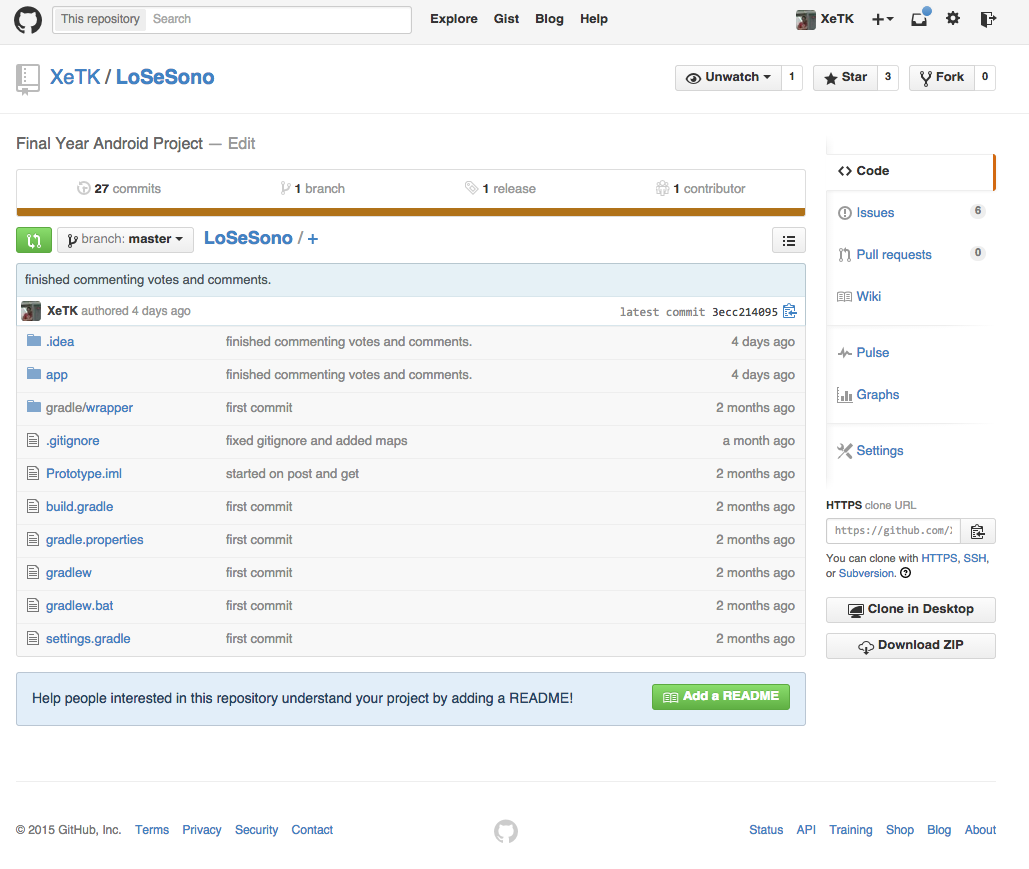
\includegraphics[width=\textwidth]{tools/github}
    \caption{Git Hub git repositories}
    \label{fig:git_hub_repos_image}
\end{figure} 

\noindent
GitHub provides an issue tracker so that users can leave issues and bug reports for the developer to fix or improve. It has been integral throughout the project to keep track of any issues that have been raised within the development of the application.\\
\\
They have been marked as fixed or left ready to be fixed in the future development of the application and gives a traceable history of any issues within the application. The UI for the issue tracker can be found in figure \ref{fig:gh_issue_tracker_image}.

\begin{figure}[H]
    \centering
    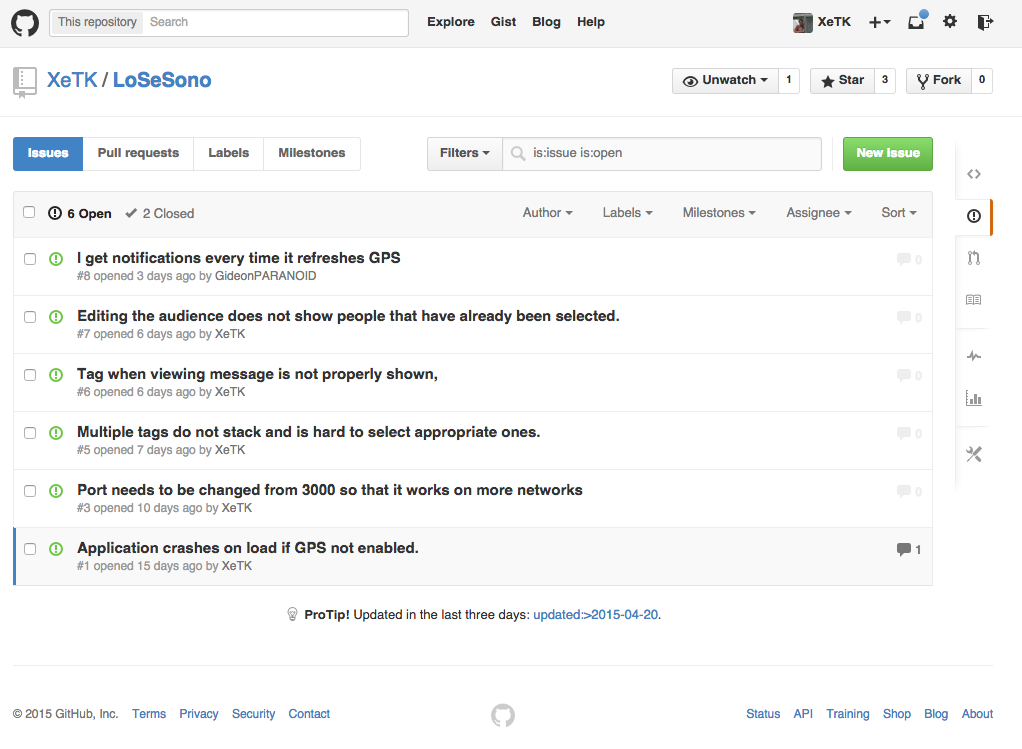
\includegraphics[width=\textwidth]{tools/githubissues}
    \caption{Github issue tracker}
    \label{fig:gh_issue_tracker_image}
\end{figure} 

\section{Android application}

This section will cover the various elements required to develop the Android Application and how the overall implementation came together.

% Alison got here


\subsection{Development Hardware}
\label{sec:dev_hardware}

The development hardware used for the project consisted of multiple phones to test the application. The primary device was a HTC One M7 running for the majority of the project Android 5.0.2. Secondary to that device there was a large chunk of development completed on a LG Nexus 4, kindly donated by Alexander Stuart, which ran Android 5.1. Further hardware consistently used were two Samsung Galaxy S2's, one a i9100 and the other a i9100p. These devices were very cheap to obtain and were very good for testing various versions of Android as they could easily be modified to suite the needs. The primary S2 that was used ran Android 4.1.2 and was completely standard. The second ran a version of CyanogenMod 11 which equated to Android 4.4.4.\\
\\
Most of the issues encountered during the development were caused by the development hardware used, as most of these devices were secondhand or lend on request, so that they were repaired and this caused a multitude of issues. At the start of the project the only device that was available was the HTC One M7 as this is my personal device. When starting the project the device ran a custom version of Android 4.4.4 which had an issue with allowing access to ADB (details of ADB can be found in section \ref{sec:adb}) which meant that deploying the application onto the device was impossible. After much toil and trying different roms and versions of Android it was possible to get the device into a state where ADB would work, but the device as a whole was not stable, thus useless for development. At this point the HTC was reverted to is prior state and the first Samsung Galaxy S2 was acquired, but this did not come without its own issues as it had Android 4.0.2 and a intermittent fault with the back button, meaning it was useless. After some research it was clear that the issue was a software problem, but tracing a standard rom for the phone proved very difficult. However, once one was acquired and the use of a Mirosoft Windows machine to flash the phone, this S2 became the test mule for the application until HTC released the 5.0.2 update for the HTC One M7, which meant the HTC became the primary phone for development.\\
\\
The two other phones used were the LG Nexus 4 and a second Samsung Galaxy S2. These came with hardware faults which had to be repaired before they could be used in the development of the application. The LG Nexus 4 had a faulty USB port so until the port was replaced charging and the use ADB were not possible as they requires the USB to work. For the Samsung Galaxy S2 more work was needed as the motherboard was heavily corroded due to exposure to water, but luckily there was a spare Galaxy S2 with a faulty screen in a box of my spares so swapping the board created one working phone.\\
\\
After theses issues development was straightforward. These issues happened within the first few weeks of the project in the configuration and setup stages, but it did eat up considerable time that could have been dedicated to development and caused many hours of frustration. It was a reminder that hardware is unpredictable and stability is not guaranteed.\\
\\
One problem that was not foreseen before the development of the project and varied heavily between devices was the ability for the device to pick up reliable GPS signals. The Samsung Galaxy S2s used had considerable problems getting a valid GPS fix. The HTC One \ & LG Nexus did a much better job of this but a lot of the time it proved very difficult to get a stable and reliable GPS fix. Thus for a large proportion of the development spoofing the location to the device was the only way to test the application.

\subsection{Environment}

The Android development environment was a large source of frustration during the development of the project as it was very difficult for get the Software Development Kit configured correctly it would often have issues with the PATH variable within command line interface which would mean ADB would become unaccessible meaning deploying and debugging the application was impossible, this would sometimes require a complete reinstall of the SDK to resolve the issue with large amount of time reconfiguring to get back to a workable state.\\
\\
There were also many issues with the Android Emulator which made it either not load or just crash unexpectedly at any point usually at a critical time within testing, due to this it was preferred to use a physical device when possible as they were much more stable and less likely to flake out during the deployment of the application but as discussed in section \ref{sec:dev_hardware} this could also be very problematic.\\
\\
One theses issues were known it was fairly easy to work around them and with a bit of patiences could be resolved fairly quickly if and when they cropped up, when everything was working correctly Android was a fairly nice platform to work with alot of robust and useful utilities for deploying and building the application, the SDK and Android Studio include all the tools to develop, compile, sign and submit full fledged applications to the Google Play store.

\subsection{Features}

This section will cover the implementation of all of the major features within the application, the subsections correspond to the functional requirements set out in chapter \ref{ch:design} section \ref{sec:functionality}.

\subsubsection*{Login}

\paragraph*{Implementation}

Login was fairly straight forward to implement most of the time was spent trying to understand the best way to keep a persistent session so that the application authenticates correctly with the backend application in a robust and reliable way to ensure that the users can readily and easily access the backend API when it is needed. The UI for the login was very simply presented and did not require a large amount work to get the application in the way detailed within the original UI mock ups. Most of the complexity within implementing the Login functionality was storing the cookies needed to authenticate the other parts of the API within the application, as when the application logs in with the credentials it is gives a cookie to say the user has been authenticated and they used this cookie to access other parts of the application.

\paragraph*{Issues}

Issues within the original implementation of the login persisted for a while till it was discovered the text that was being entered into the dialog was not being parsed correctly to remove any spaces that were residing at the end of strings causing issues with the login as the usernames would have spaces at the end and when comparing the strings on the server side with the usernames of the user it would not match, This seems to come down to the Android implementation of text boxes where it will automatically add a space after a word as it thinks its very likely another word will come after it.


\subsubsection*{Registration}

\paragraph*{Implementation}

Implementation of registration was very straight forward it was more straightforward to implement than login as it does not require the extra work needed to create a cookie and consists of just sending a straight HTTP POST request to the server to register the user correctly, the users details are passed over HTTP POST parameters and then the server registers and authenticates the user. UI implementation was kept the same as the mockups so was straight forward with no problems.

\paragraph*{Issues}

The same issue with text boxes was present within the implementation of the the Registration functionality where Android automatically added a space to the end of each field automatically when it thought that the field would have another word after the users details. This was fixed with some simple trim commands being issued on the text that was contained within the text boxes to remove any trailing spaces that would cause the registration to fail.\\
\\
A fairly major issue arose with the development in registration, this issue was more to do with the server side of the application but caused issues within the UI, the issue was caused by the backend application returning a failure code when successfully registering the user which would cause the UI to show a error rather than completing as expected and the UI would not return back to application because it thought it had failed, once this issue was resolved within the backend then the UI performed as expected.


\subsubsection*{Adding Friends}

\paragraph*{Implementation}

The implementation of the adding friends UI was fairly similar to the login and registration it did not present any issues it used the restful service that uses the cookies to authenticate the user with the backend API.

\paragraph*{Issues}

Similar issues with Login and Registration persist with the trailing space on text boxes, lack of user feedback when adding a friend and the fact the application automatically accepts any request at this point is a major issue and will be implemented within further development of the application.


\subsubsection*{GPS Location}

\paragraph*{Implementation}

GPS implementation was fairly straightforward there was a fair bit of reading over the subject and there was a very well written StackOverflow post \cite{mudit:HowdoIgetthecurrentGPSlocationprogrammaticallyinAndroid:2009:online} that detailed fully how to access the GPS API's within the Android operating system and to get the location effectively and reliably, this API will need some work to be used within a production environment the core functionality is there but the optimisation to ensure the devices battery is not depleted to rapidly is not implemented at this point and will be a point of further development to ensure that in a production environment the users do not get annoyed. Figure \ref{fig:battery_issues} shows the usage of the application after a typical day and understandably without the optimisation it uses a lot of the phones battery.

\begin{figure}[H]
    \centering
    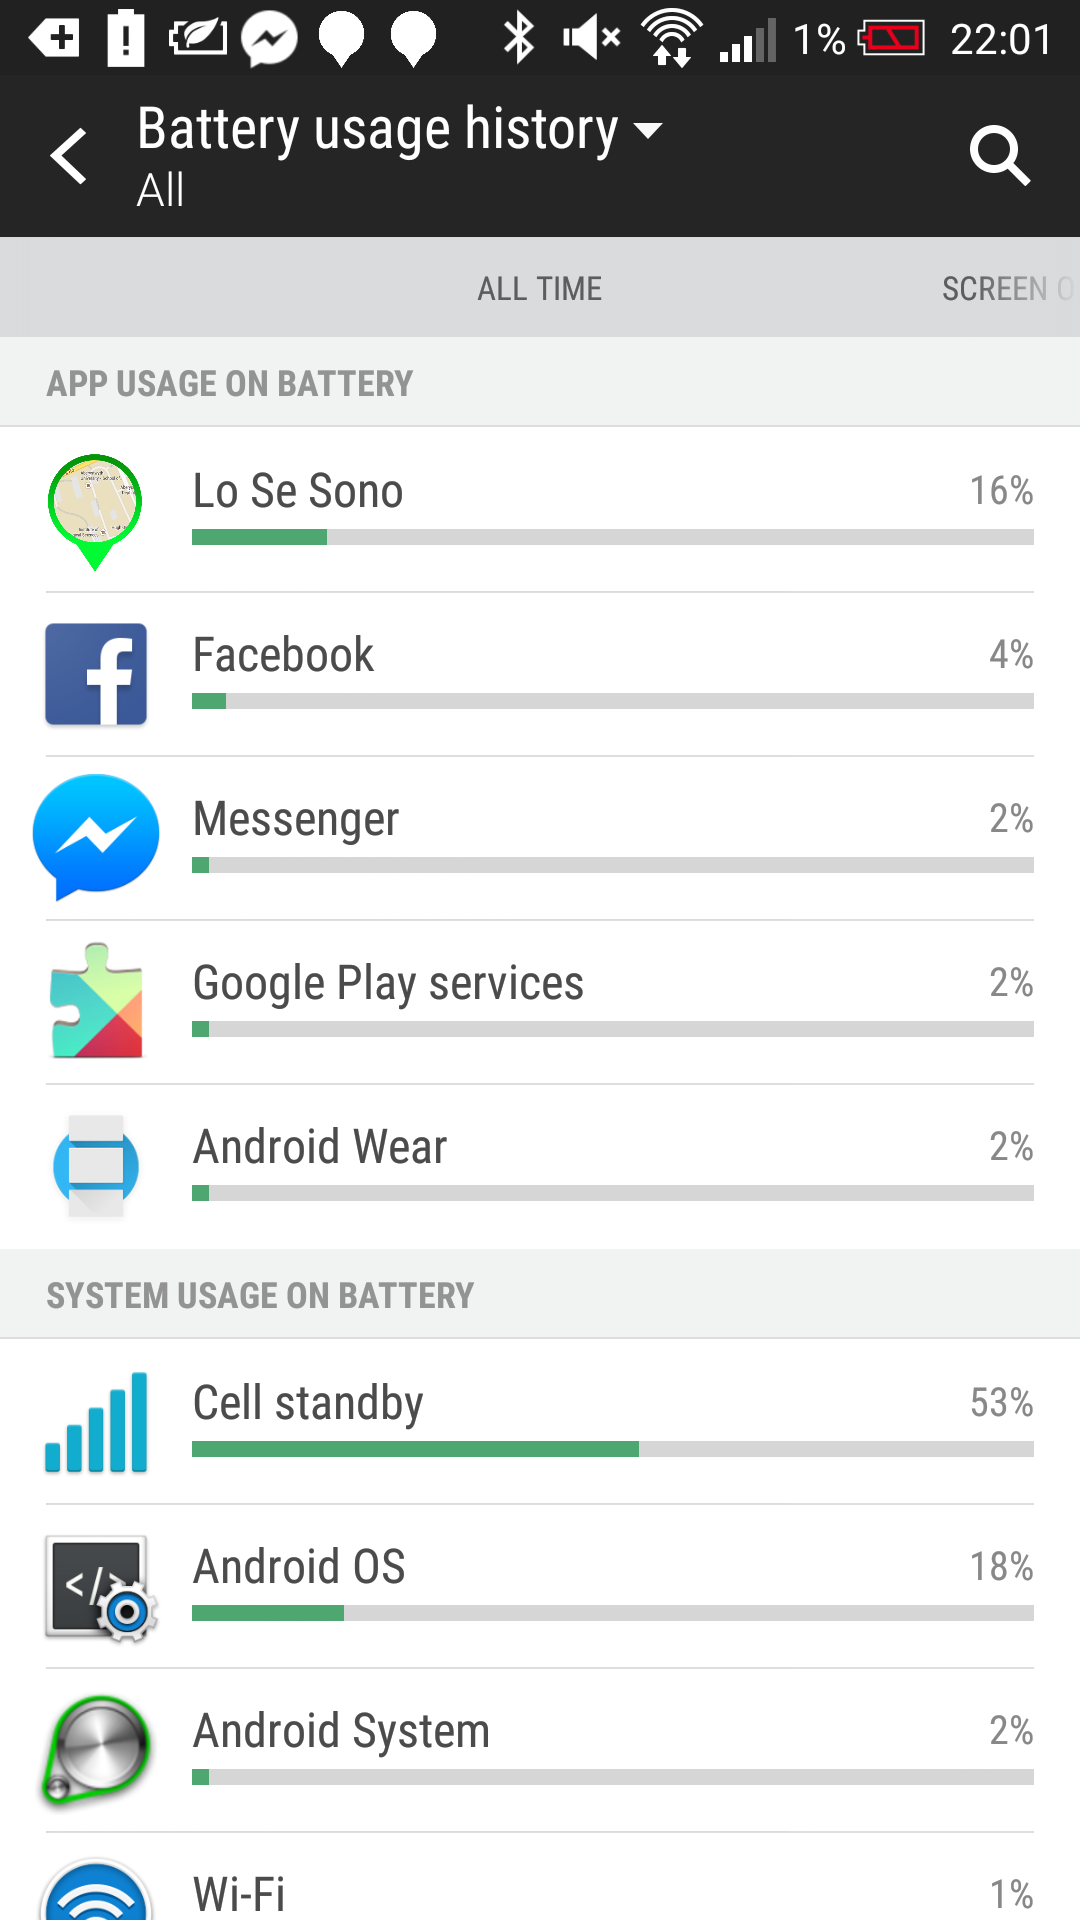
\includegraphics[width=0.5\textwidth]{batteryissues}
    \caption{This shows the application battery usage after a average days use}
    \label{fig:battery_issues}
\end{figure} 

\paragraph*{Issues}

Major issue with the GPS API that is being used is that if GPS is not enabled when the application starts up then the application will crash, this again is another issue that will be resolved within further development of the project and is most likely a small over site within the implementation of the UI or where it is used within the application. There was some small issues with implementing the code that calculates the distance between two GPS coordinates as the algorithm it was devised from one written in JavaScript and converting it to Java was fairly difficult due to the lack of explanation of what was happening.


\subsubsection*{Maps}

\paragraph*{Implementation}

The Google maps implementation within the application was one of the more difficult elements of the application to implement this was mostly down to the documentation for the API being fairly out dated and using deprecated functionality within the UI, this was resolved with some reading of some StackOverflow posts and disassembling the API to find the new functions for pulling up and executing the code once the UI had fully render and loaded. 

\paragraph*{Issues}

There were some issues with getting the tags to show in the correct places and if there is multiple tags on the same location then it is very difficult to differentiate between different tags that are all in the same location, as they all clump together and make it very difficult to self the marker that is wanted. There is also some issues with the text rendering and labels in the current where it does not display the text correctly.


\subsubsection*{Posting message}

\paragraph*{Implementation}

Once Mapping and the GPS had been implemented sufficiently it was fairly easy to implement posting of messages as it took characteristics from Mapping, GPS and Adding Friends to create using the mapping to show the current location on the map, GPS to gather the current location and the adding of friends to enable the sending of the RESTful request to the server the code from theses features works together to create the adding of a friend. This shows the progression throughout the development of the application as features build on top of each other to enable the next feature to be more mature and fully fledged.

\paragraph*{Issues}

Issues within the implementation are down to the way that the requests are structured as submitting the messages goes first then one it has been submitted the user binds the friends to the user, where as this should realistically be done at the same time rather than sequentially this is a minor issue and should be resolved in further development. Other issues were trying to layout the screen in a effective manor that everything can be viewed efficiently without disappearing of the screen on smaller devices this has worked to some degree but still has issues and this will be resolved within further optimisation of the application when it enters a production like state.

\subsubsection*{Retrieving messages}

\paragraph*{Implementation}

Again this builds upon the posting of messages and uses a very similar layout in screen design where it has a map showing the comment left on the location it is fairly straight forward to pull the information needed and add it to the tags on the map with the information needed. 

\paragraph*{Issues}

Again major issues were down to layout and getting all of the relevant information on the screen at one time, with the comments and voting it makes the screen very complex. There is also some issues with rendering the page as the requests are doing via AJAX and also done sequentially means that bits of the screen loads and renders at different times which can be a tad confusing for the users this should be cleared up with a bit more development to the screen.

\subsubsection*{Retrieving notifications}

\paragraph*{Implementation}

The implementation for processing and receiving notifications within the application was a fairly difficult and time consuming part of the application to get working. The route given by the Android SDK documentation was very out dated and caused a multitude of issues in getting the correct behavior for the notification, once the large underpinning structure of the notifications code was implemented it became much similar and it was very easy to get the correct behavior when the events were triggered within the UI.

\paragraph*{Issues}

There were some difficult points with implementing the notifications mostly due to inadequate and out of date tutorial's and documentation on the subject there was a lot of time spent trying to piece various tutorials and bits of API documentation together to get a working solution. Issues still persist into the current version of the code, which boils down to not checking correctly if a notification already exists and also partly down to messages not being marked correctly server side to say they have already been read by the user.

\subsubsection*{Comments}

\paragraph*{Implementation}

Comments were a very interesting concept to implement within the application, it was fairly complicated to get all of the UI elements lined up correctly and to display all of the relevant information that is needed for correct interpretation of comments. Creating custom UI elements and reusable sections to add into the page to create a consistent theme for all of the comments, the commenting and voting functionality is very closely linked and the share the same screen space and getting them all to render effectively and in a readable state was fairly complicated. Although this was a fairly fun and simplistic part of the functionality to implement, it will require more work to get it to work correctly on all different screen sizes but this is a point to be considered for further development.

\paragraph*{Issues}

For the implementation of the comments feature there was not many issues, most of the time during the implementation of this feature was spent trying to get the UI elements to be positioned in the correct places and to scale correctly. The complexity of UI design in this area and integrating the UI to the background code was complicated mostly due to how many fields and how dynamical all of this section is.

\subsubsection*{Votes}

\paragraph*{Implementation}

The implementation of votes took after comments and was carried out at the same time as implementing comments as they share the same screen space and UI area, The structure behind voting is very similar to the comments where it sends a request to the backend to increment the amount of votes there are for a given comment or message.

\paragraph*{Issues}

As it stands the major issue with votes is that there is no way to refresh just one vote on the screen and it is required to refresh all of them to get the new details about the comment or message, this has been badly implemented in the UI so that if the button is pressed the value is updated but it may not reflect what is held in the backend due to the difficulty of refreshing just one region of the screen this will be fixed in future development.

\section{Server side application}

This section covers the overall implementation and setup of the backend services required to get the application working, it will not talk about design this is covered in chapter \ref{ch:design} section \ref{sec:server_side_design}.

\subsection{Environment}

This section covers the environment the application will be run in with the server side. The development environments slightly from the technologies covered in this section, instead of a Linux based machine running the application the development system used is a Apple Mac, this should not create any issues as the technologies chosen are highly portable and work on many different operating systems.

\subsubsection{Debian based Linux}
\label{sec:debian_server}

For running the server side services it was decided that a Linux based server would be the best as it offers the flexibility needed to run all the applications and services needed to get application working as intended. Due to prior knowledge of Debian based distributions it was decided to use a strictly Debian based server as the test server, and due to some stability issues for the production server to use Ubuntu Server 14.04.\\
\\
The justification of two servers comes down to trying to emulate the the structure that most company use of having a server for testing the application so that test data does not get put into a production environment and cause issues within the production environment. It is fairly fundamental that production users data is not mixed in with the development and test data as this could cause confusion and make it harder to see what is a test and what is actual user data. Segregating testing and production is also integral for testing as production users can be left on the stable platform in production till the version in test has been fully tested and proven to be stable where it can then be moved to the production server for the users to use.\\
\\
Both of the server installations used are provided by Digital Oceans which is the hosting service that was chosen to run the application this decision was covered in details in section \ref{sec:digial_oceans}. Each of the installations had only the bare essentials installed on them to get the application working this should help with stability and mean that we are not wasting space, the frameworks and applications chosen to be installed on the servers were PostgreSQL and Node.js theses are the two core components to the backend application for this project.\\
\\
Deployment of both of the servers was relatively painless there was very small issues with version mismatches with the PostgreSQL version used within the development environments but once this was fixed there was no issues with the deployment of the applications on theses systems.

\subsubsection{PostgreSQL Database}

PostgeSQL is fairly complicated to configure correctly, it required a fair amount of reading of the PostgreSQL documentation \cite{Postgres:APIDocumentation:2015:online} to ensure the application was configured correctly, this was teamed with some versions mismatches the version within the Debian repositories was a few versions older than the most current and did not have some of the more advanced features that were being used within the application, in particular the JSON manipulation tools. To fix theses issues it required compiling PostgreSQL from the source code to ensure we had the correct version on the server.\\
\\
For the encryption used within the application extra modules need to be installed within the PostgreSQL installation and registered this was fairly hard to find documentation on but it was found within a StackOverflow post \cite{se:howtoinstallpgcrypto:2011:online}. 

\subsubsection{Node.js environment}

It was decided for Node.js to ensure that the systems were running the latest version of the software that it would be wise to download the latest stable version from the Node.js website \cite{nodeteam:node:2015:online} this is supplied in a source code, it would then be compiled on the systems to ensure that they had the most up to date version of the software. It was fairly easy to compile and configure Node.js without any issues this was likely due to having done it in the past, next attention was set to getting the application running on the server with Node.js running after cloning the backend code onto the server it was simple enough to run 'npm install' and it would automatically pull all of the external libraries needed from the cloud using the Node Package Manager(NPM), NPM helps with deployment of the application and is good for keeping track of the Node.js applications running showing any exceptions or stack traces if the application falls over with a log file to give the full picture if something happens.\\
\\
Overall working with Node.js is very straightforward and enjoyable it gives a lot of freedom and has a large variety of libraries and packages that can be used to improve the application and saves reinventing the wheel. The language JavaScript that Node.js is implemented in allows a lot of flexibility to how functionality is implemented this coupled with the large arrange of 3rd party libraries and code bases to implement the functionality required by the user, for a fairly young environment it is very mature and used by fairly large organisations like the British Broadcasting Corporation or Walt Disney gives confidence it is a very competent platform building applications.

\subsubsection{Digital Ocean Droplets}
\label{sec:digial_oceans}

For hosting the application Digital Ocean was chosen to be the company that hosted the application as they gave \$100 worth of hosting free to students through the Github Education bundle but it could of quite easily been any other of the big hosting companies for example HostGator or Gandi. The service given by Digital Oceans has been exceptional, they have the ability to spin up a virtual private server(VPS) or as they call it a Droplet in a matter of minutes and even give the options to have Node.js and PostgreSQL installed at the time the Droplet is created which is a great time saver.\\
\\
The customers service has been very good with helping with issues, as explained in section \ref{sec:debian_server} there were some issues with the PostgreSQL installation on Debian due to out of date repositories there representative gave a quick and well explained answer on how to upgrade and install the newer version of PostgreSQL they also gave advice on how to resolve a memory issue caused by the projects middle tier application. Although the memory issue has not been resolved the allocation of more memory has made the issue happen less frequently and this issue should be resolved during further development. The ability to dynamically resize the requirements of the server is a great help when debugging various issues and can help quickly when an application is under heavy load and means the owner of the application can decide when they need to to upgrade the capacity of the application depending on the situation that is occurring with the application at that time.

\subsection{Middle tier application}

This section will cover the implementation of the various parts of the middle tier application.

\subsubsection{Core functionality}

The spike work for the development of the middle-tier got of to a bad start with the wrong choice of framework making development problematic, how this issue was resolved in detail can be found in section \ref{sec:node_choice_of_tech}.\\
\\
After initial spike work implementation of the core structure of the middle tier was fairly straight forward and there was no show stopper while implementing the system, there were a few minor issues during the development of the middle tier, mostly down to badly written API documentation that did not fully explain the constructs of the library that was being used.\\
\\
There has been a few issues with trying to setup tests correctly to make sure that the API authenticates correctly with the client it took a few attempts to find a library that was capable of storing cookies correctly and parsing them and re-injecting into the header of other requests to authenticate the user.\\
\\
As it stands some of the functionality of the backend is incomplete there is no error handling for when things go wrong and this will be implemented within further development of the application. Again it should be noted that the authentication within the application as it stands is not up to a standard that could be used within a production environment.
\\
% -- write more maybe?

\subsubsection{RESTful Interface}

Implementing the RESTful interface within the application was fairly straight forward due to how the application has been designed where various URL routes are loaded dynamically so that as the various sections of the application can be implemented when they are needed and do not require changes to the rest of the application to implement the new URL route for the new functionality.\\
\\
There is one issue with the HAPI.js API that causes issues with the implementation if for example the application is working with a POST request and it the status of the request is successful there is a HTTP status for successful so replying to the server "reply('success');" will cause a 302 error code which the client interpret as a error and the client will fall over.\\
\\
The standard HAPI.js postRoute and getRoute have been overwritten within the design so that they are always secured when they are used within the application, as they have been overwritten to ensure that the developer always uses protection on the routes within the application. The implementation of security within the application was a provided by a mixture of external libraries and custom code to interface with the database to ensure that the user is entitled to access the application, it has been fairly straight forward to amalgamate this code together to provide the functionality needed to authenticate the user although this could be considered a weak spot for the authentication of the application as it was not written by a security expert and may be prone to errors.\\
\\
One small oversight at the time of developing the was that JSON objects do not encapsulate other useful objects that are used within the same function thus in the current design the user will be returned a user\_id and then will have todo another rest call to get the user object for the user\_id it had received rather than having the user object encapsulated in the first request.

\subsubsection{Database Connector}

The use of Sequelize \cite{SaschaDepold:Sequelize:2015:online} to act as a connector between the HAPI.js application and the PostgreSQL database may have been a bad decision due to the memory allocation issues caused by it. It may also be adding extra complexity where it is not needed as it is a object relational mapping type of framework and in the implementation of the application it is not being utilised at all and the use of raw queries is used instead that is passed through the API to the SQL engine to execute. A framework that would be better suited to the job may be node-postgres as this is a much smaller API that interacts with the postgreSQL engine and does not have the extra layer of complexity of an Object Relational Mapper on top of it.\\
\\
Implementation with Sequelize was fairly straightforward though as it gave all the features required to work with the database within its bounds of the framework, it gave nicely formated JSON object containing the information from the query and theses could be directly sent to the client without any manipulation at-all which helped cut down the complexity of editing and formatting the data in-between the database and the client.

\subsection{Database level}

This gives a overview of the implementation of the database for the project.

\subsubsection{Tables}

Implementing the tables was fairly simple and straight forward for the most part as the original design stayed the same throughout although with a few very minor changes to add in functionality that was was not assessed at the beginning of the project. Changes were made when some minor issues with the constraints placed on a table were not correct making it impossible to insert the correct data into the database. Modifications to the structure are discussed more in-depth in chapter \ref{ch:design} section \ref{sec:database_strucutre}.\\
\\
Some changes were made later in the implementation of unique data was inserted along with the constraints to check that the wrong values were not inserted into the database, the referencing between different columns also caused some issues during development as in the early stages of development there was a need to clear the tables to ensure that bad data was removed and would not interfere with the new data being inserted, the issues arise when trying to truncate the tables to give a fresh dataset to work with, truncating the tables would lead to a constraint error that would prevent the data being deleted as it thought there may still be references left in the other table that depend on the other references, this issue was overcome by using delete rather than truncate "truncate table messages" would fail but "delete from messages where 1 = 1" would complete without error.

\subsubsection{Functions}

Functions within the database were a great time saver in the implementation of the application as functions could be written in the database to do checks to ensure that the data being inserted was correct, along with writing functions to validate that the authentication details are correct without pulling data out of the database and doing a context switch between the SQL engine and the Node.js application which will ultimately slow down the application dramatically if it has to do a lot of context switching.\\
\\
The implementation of the database function was fairly straight forward after the first one was implemented, there was some issues due to this being the first time using PostgreSQL but it was quickly sorted after a few functions had been implemented and difference between PostgreSQL and PL-SQL had clicked. PostgreSQL functions were one of the most interesting concepts that was used throughout the development of the application as it helped with speeding up the application and ensuring that the data inserted into the database was validated and manipulated correctly before being inserted into the database, the slight oddity with how functions is called took a while to get over to run a database function within the SQL engine you must issue a SELECT command for example "select function\_name('some','data');" which was a little unusual.\\
\\
Triggers in PostgreSQL are implemented very slightly differently than PL-SQL which took a while to understand but all the issues with the implementation of various features in PostgreSQL were easily answered by referring to the API documentation \cite{Postgres:APIDocumentation:2015:online} for the SQL engine.

\section{Review of implementation}

The implementation of the project as a whole was straight forward overall of course with any large project there were small patches of development where the development was slowed down due a problematic and complicated issue that required a large amount of time to be spent on it to overcome the issue.\\
\\
HAPI.js and PostgreSQL where a pleasure to work with and caused very minimal issues they were great frameworks that lead them selfs to build a robust and well structured backend API for the application as a whole.\\
\\
Android on the other hand had a lot of issues that caused delays to the development this could be put down to that Android was a new framework to work with and the developer did not have any prior knowledge but also a large proportion can be put down to the oddities of the environment and nuances in hardware which is covered at the start of this chapter in section \ref{sec:dev_hardware}.
